% Draft sections: Materials/Methods + Experiments/Results + Discussion.
% This file is content-only and is intended to be \input{} into docs/cmc/main.tex.

\section{Materials and Methods}
\label{sec:methods}

\subsection{Datasets and Protocol Variants}
\label{sec:datasets}

Because the study moves from public-benchmark evaluation to a low-resource target domain, the dataset description needs to clarify not only the available labels but also the distinct role played by each dataset. The VSB-derived dataset is used to define the in-domain benchmark and broader protocol analysis, whereas VNWoodKnot is used as the external target domain for adaptation experiments. Figure~\ref{fig:dataset-overview} provides a visual comparison, and Table~\ref{tab:dataset-comparison} summarizes the main quantitative differences that later motivate the domain-shift analysis.

\begin{figure*}[t]
  \centering
  \begin{subfigure}[t]{0.48\textwidth}
    \centering
    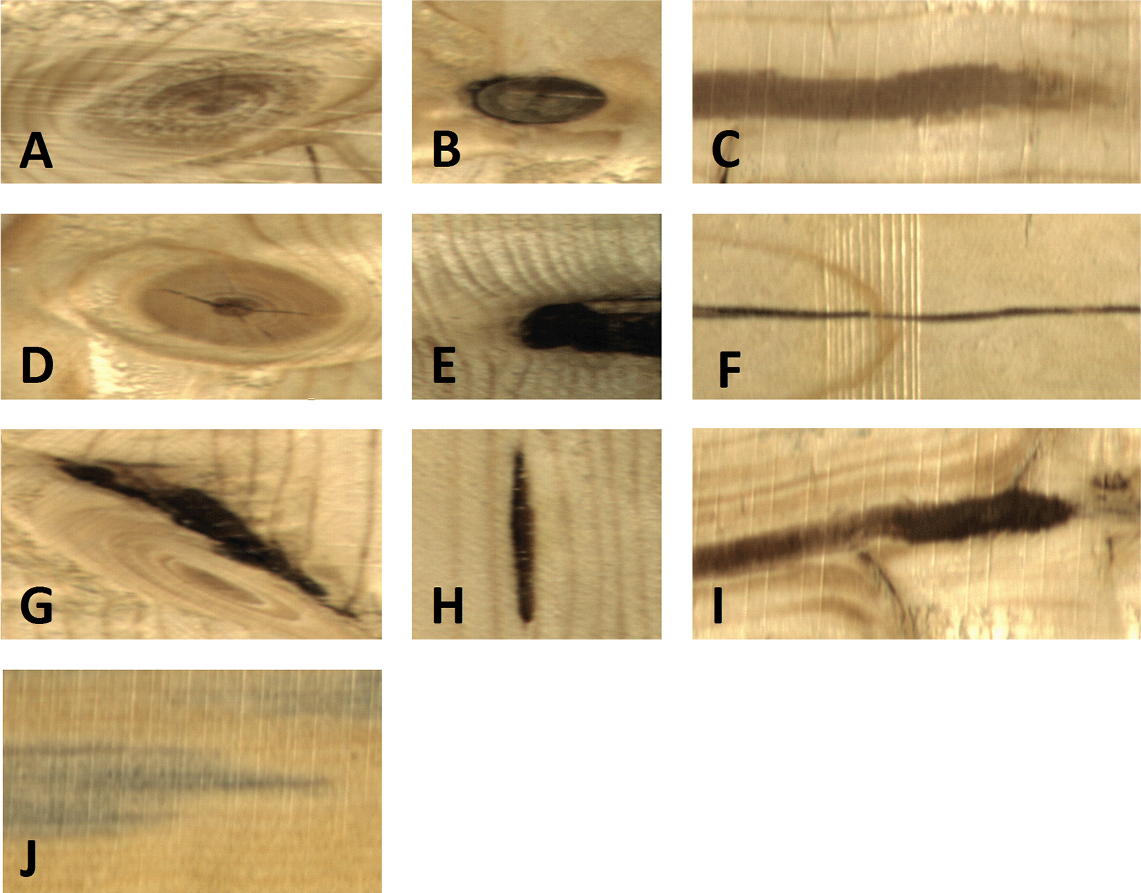
\includegraphics[width=\linewidth]{figures/wood_defect_types.png}
    \caption{Representative defect categories from the public benchmark domain. The original dataset includes ten defect types, from which the seven-class protocol used in this study is derived \citep{kodytek_dataset}.}
    \label{fig:dataset-overview-public}
  \end{subfigure}\hfill
  \begin{subfigure}[t]{0.48\textwidth}
    \centering
    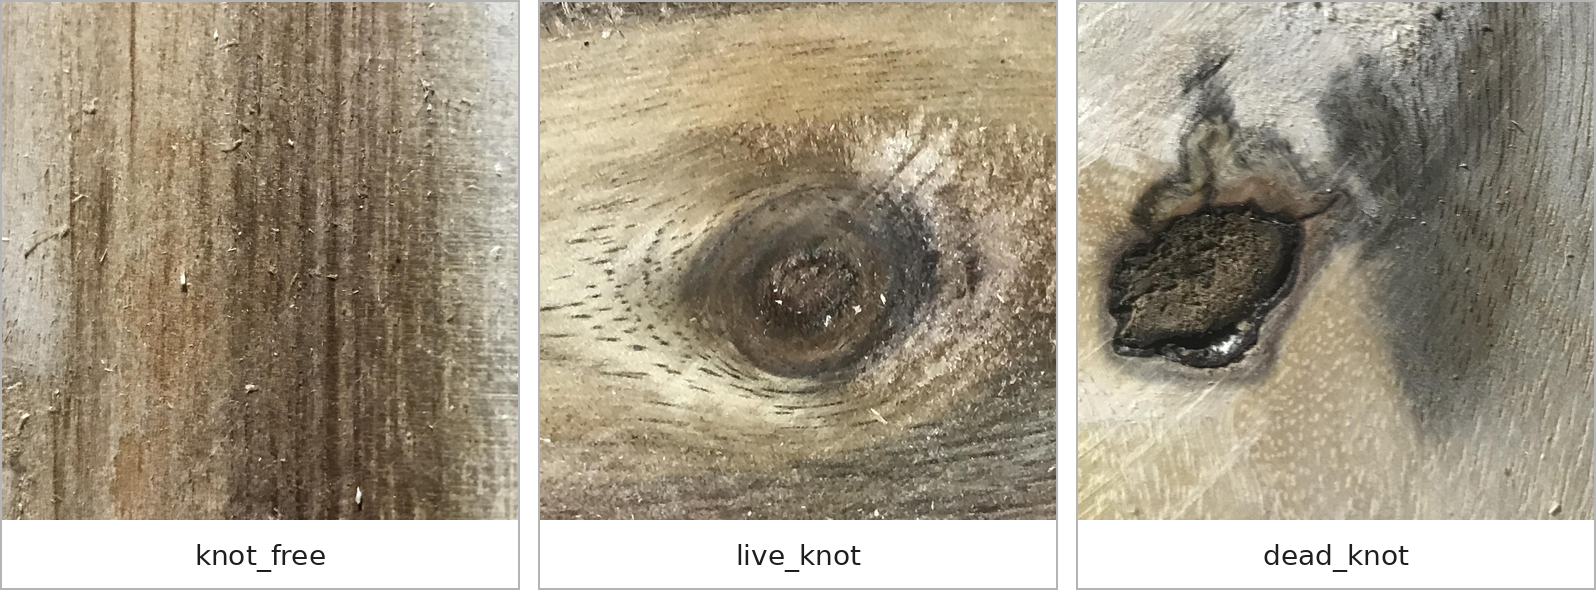
\includegraphics[width=\linewidth]{figures/vnwoodknot_triptych.png}
    \caption{Representative images from VNWoodKnot, showing the three labels available in the original dataset: \texttt{knot\_free}, \texttt{live\_knot}, and \texttt{dead\_knot}.}
    \label{fig:dataset-overview-vn}
  \end{subfigure}
  \caption{Visual comparison of the two datasets used in this study. The left panel represents the public source domain used to construct the screened and broader in-domain protocols, while the right panel shows the low-resource target domain used for supervised adaptation experiments. The contrast in defect scale, framing, and label structure is one of the central motivations for the comparative evaluation.}
  \label{fig:dataset-overview}
\end{figure*}

\paragraph{Public benchmark domain: VSB-derived dataset.}
The in-domain experiments are built on the large-scale wood surface defect dataset of Kodytek \textit{et al.} \citep{kodytek_dataset}. From this source, we derive a seven-class label space consisting of \texttt{live\_knot}, \texttt{dead\_knot}, \texttt{resin}, \texttt{knot\_with\_crack}, \texttt{crack}, \texttt{marrow}, and \texttt{knot\_missing}. This shared label space is used for both the screened benchmark and the broader in-domain protocol so that protocol sensitivity can be analyzed without changing the task definition.

\paragraph{Low-resource target domain: VNWoodKnot.}
VNWoodKnot is used as the external target domain. Compared with the public benchmark, it is substantially smaller and visually more homogeneous, with fixed-size images collected under a different acquisition setting. The original VNWoodKnot label space contains \texttt{knot\_free}, \texttt{live\_knot}, and \texttt{dead\_knot}. In our study, the two knot classes form the detection task, while \texttt{knot\_free} images are preserved as negative samples. This makes VNWoodKnot a practically relevant low-resource target domain for evaluating supervised adaptation rather than a direct seven-class benchmark.

\paragraph{Protocol A: Screened seven-class benchmark (\texttt{vsb7\_3600\_rarefirst}).}
We define a screened benchmark intended to be comparable in spirit to prior seven-class screened subsets derived from the Kodytek dataset \citep{kodytek_dataset}. The benchmark is constructed by selecting a fixed number of source images and then generating tile records for detection training and evaluation. Under our YOLO export for this benchmark, the split contains 7,679 train tile images, 977 validation tile images, and 972 test tile images.

\paragraph{Protocol B: Full seven-class protocol (\texttt{full\_7class}).}
To test whether screened-benchmark conclusions remain valid under a broader in-domain setting, we also evaluate on a full seven-class protocol constructed by filtering the full dataset down to the same seven classes. This protocol produces a larger validation split with 4,846 validation tile images under the current tiling setup. In addition to the original 20-epoch run retained as the stronger internal reference under our study evaluator, we also use an additional 200-epoch YOLO rerun as a diagnostic schedule check.

\paragraph{External protocol: VNWoodKnot adaptation setting.}
For the external study retained in this manuscript, VNWoodKnot is reformulated as a two-class detection task containing \texttt{live\_knot} and \texttt{dead\_knot}, while \texttt{knot\_free} images are preserved as negatives. This setting allows us to measure how quickly a screened-source checkpoint can adapt to a target wood-inspection dataset under a fixed fine-tuning budget.

\subsection{Dataset Analysis and Domain Shift Indicators}
\label{sec:data-analysis}

The visual differences in Figure~\ref{fig:dataset-overview} are reflected by substantial quantitative differences between the two datasets. These differences matter because the source benchmark mainly tests small-defect localization under a richer seven-class taxonomy, whereas the target domain emphasizes larger knots under a much smaller label space. Table~\ref{tab:dataset-comparison} summarizes the main characteristics that shape this mismatch.

\begin{table*}[t]
  \centering
  \caption{Comparison between the public benchmark domain and the low-resource target domain used in this study.}
  \label{tab:dataset-comparison}
  \footnotesize
  \setlength{\tabcolsep}{5pt}
  \begin{tabularx}{0.94\textwidth}{>{\raggedright\arraybackslash}p{0.24\textwidth} >{\raggedright\arraybackslash}X >{\raggedright\arraybackslash}X}
    \toprule
    Attribute & Public benchmark domain (VSB-derived) & Low-resource target domain (VNWoodKnot) \\
    \midrule
    Role in this study & Source benchmark for in-domain comparison, protocol-sensitivity analysis, and source pretraining & External target domain for supervised adaptation under limited data \\
    Source images & 20,276 & 1,515 \\
    Box annotations & 43,974 & 1,021 \\
    Label space used in this study & 7 classes: \texttt{live\_knot}, \texttt{dead\_knot}, \texttt{resin}, \texttt{knot\_with\_crack}, \texttt{crack}, \texttt{marrow}, \texttt{knot\_missing} & 2 detection classes (\texttt{live\_knot}, \texttt{dead\_knot}) with \texttt{knot\_free} retained as negatives \\
    Image format & Heterogeneous source images converted into tiled training/evaluation records & Fixed-size images ($1500 \times 1500$) \\
    Derived tiles / processed images & 48,156 tiles after preprocessing (38,493 train / 4,879 val / 4,784 test) & No tiling used in the reported target-domain setting \\
    Empty / background-only images & Not emphasized in the benchmark protocol & 500 \texttt{knot\_free} images \\
    Mean normalized bbox area & 0.008857 & 0.119985 \\
    Small-annotation ratio & 75.95\% (33,400 / 43,974) & 0\% (0 / 1,021) under the same rule \\
    Main implication & Strong emphasis on small-defect localization and long-tail multi-class discrimination & Stronger emphasis on larger knot regions, simpler label space, and source-to-target transfer \\
    \bottomrule
  \end{tabularx}
\end{table*}

\paragraph{In-domain dataset size and tiling.}
The in-domain dataset audit reports 20,276 source images and 43,974 box annotations. Under the tiling pipeline used in this study, these source images yield 48,156 tile images, with 38,493 train / 4,879 validation / 4,784 test tiles. This tile-based protocol is the basis for all in-domain training and evaluation.

\paragraph{Small-defect prevalence (in-domain vs external).}
Small objects dominate the in-domain dataset: 33,400 out of 43,974 annotations (75.95\%) satisfy the same small-defect rule used in our evaluation summaries. In contrast, VNWoodKnot has effectively zero small annotations under that rule (0 out of 1,021). This implies that the in-domain task is heavily influenced by small-defect localization, whereas VNWoodKnot emphasizes larger knot boxes.

\paragraph{Bounding-box scale mismatch.}
The mean normalized bounding-box area in the in-domain dataset is 0.008857, whereas VNWoodKnot has a mean normalized bounding-box area of 0.119985. This order-of-magnitude gap indicates a strong difference in object scale and framing. Together with the label-space reduction and the presence of many negative images in VNWoodKnot, these statistics support interpreting the external evaluation as a substantial source-to-target shift rather than as a minor threshold-calibration issue.

\subsection{Detector Variants}
\label{sec:detectors}

Based on the defect characteristics discussed in Sections~\ref{sec:introduction} and \ref{sec:data-analysis}, we select three detector families to cover complementary operating points in a practical wood-inspection design space. First, Faster R-CNN with MobileNetV3-FPN provides a proposal-based two-stage family that combines explicit region refinement with lightweight backbones, making it a relevant reference when localization control and computational efficiency must be balanced \citep{faster_rcnn,mobilenetv3,mittal_2024}. Second, YOLOv8s represents a compact one-stage family that has become a strong practical default in recent defect-inspection and wood-defect studies because of its favorable speed--accuracy trade-off and multiscale dense prediction behavior \citep{ultralytics_yolo,odca_yolo,bpn_yolo,sim_yolo,fdd_yolo}. Third, we test two targeted YOLO refinements, namely a higher-resolution P2 head and a WNIoU-style localization loss, because high-resolution detection layers and alternative regression losses are among the most common responses to small-object and unstable-localization problems in current detection literature \citep{wei_2024_smallreview,hua_2025_smallsurvey,cmc_insulator_small,cmc_msese}. This detector selection allows the study to address two practical questions at once: which detector family is most suitable for the present wood-defect setting, and whether widely motivated small-object-oriented refinements materially change that ranking.

\paragraph{Low-capacity MobileNet baseline (\texttt{baseline\_detector}).}
The lowest-capacity reference in our study is a Faster R-CNN detector instantiated from \texttt{fasterrcnn\_mobilenet\_v3\_large\_320\_fpn} with the image size fixed to $1024 \times 1024$. We include this model as a lower-cost anchor point for the proposal-based family, so that the study can distinguish between the effect of detector family and the effect of simply scaling backbone capacity inside the same two-stage design \citep{faster_rcnn,mobilenetv3}.

\paragraph{High-resolution MobileNet baseline (\texttt{MobileNet\_HR}).}
The main lightweight family in the paper uses Faster R-CNN + MobileNetV3-Large-FPN, instantiated from \texttt{fasterrcnn\_mobilenet\_v3\_large\_fpn} and trained at $1024 \times 1024$. This family appears in \texttt{baseline\_mobilenet\_hr\_full\_7class} and the screened-benchmark variants \texttt{E0}, \texttt{E1}, and \texttt{A1}. We use it as the principal lightweight two-stage reference because it retains the proposal-based refinement behavior of Faster R-CNN while providing a stronger MobileNet backbone than the lower-capacity baseline above \citep{faster_rcnn,mobilenetv3}.

\paragraph{YOLOv8s baseline (Y0).}
\texttt{Y0-full\_7class} and the screened compact YOLO branch use the standard YOLOv8s architecture with pretrained weights (\texttt{yolov8s.pt}) in the Ultralytics implementation \citep{ultralytics_yolo}. We choose YOLOv8s as the compact one-stage baseline because it provides a modern, strong, and deployment-relevant detector family that is close in spirit to the YOLO-style models dominating recent wood-defect literature \citep{odca_yolo,bpn_yolo,sim_yolo,fdd_yolo}. The final reported screened run is denoted \texttt{Y0-3600e200}.

\paragraph{P2-head ablation (Y1).}
\texttt{Y1} adds an extra P2 detection head to YOLOv8s via a modified model configuration (\texttt{yolov8s-p2-7class}). This variant is motivated by a task-specific hypothesis: several wood defects in the present benchmark occupy small image regions or exhibit weak local contrast, so discriminative cues may be attenuated when prediction begins only from coarser pyramid levels. Adding a higher-resolution detection layer therefore tests whether earlier multiscale prediction improves the representation of small defects in this domain, as suggested by recent small-object detection studies \citep{wei_2024_smallreview,hua_2025_smallsurvey,cmc_insulator_small}. In the present study, \texttt{Y1} serves as a screening-stage test of whether resolution-oriented refinement can materially improve the compact YOLO baseline.

\paragraph{WNIoU-style box-loss ablation (Y2).}
\texttt{Y2} modifies the box regression loss to a WNIoU-style hybrid loss. In this implementation, the loss is a weighted mixture of a CIoU term and an NWD-like term, with an additional focusing factor. This variant addresses a different hypothesis from \texttt{Y1}: some wood defects, particularly thin cracks and irregular knot-related regions, may be limited less by feature resolution than by unstable geometric supervision during box regression. A distance-aware and reweighted localization loss is therefore tested as a compact way to improve localization robustness without modifying the detector architecture itself \citep{wei_2024_smallreview,hua_2025_smallsurvey,cmc_msese}. In the present study, \texttt{Y2} serves as a screening-stage test of whether loss-level refinement alone can improve the compact YOLO baseline on the screened benchmark.

\begin{table}[t]
  \centering
  \caption{Detector families covered in the study.}
  \label{tab:detector-families}
  \footnotesize
  \setlength{\tabcolsep}{4pt}
  \begin{tabularx}{\linewidth}{>{\raggedright\arraybackslash}p{0.16\linewidth} >{\raggedright\arraybackslash}p{0.28\linewidth} >{\raggedright\arraybackslash}p{0.23\linewidth} X}
    \toprule
    Family & Implementation & Representative runs & Role in study \\
    \midrule
    MobileNet-low & Faster R-CNN + MobileNetV3-320-FPN & \texttt{baseline\_detector} & exploratory low-capacity reference \\
    MobileNet-HR & Faster R-CNN + MobileNetV3-Large-FPN & \texttt{B1}, \texttt{E0}, \texttt{E1}, \texttt{A1} & lightweight high-resolution baseline family \\
    YOLO baseline & YOLOv8s & \texttt{Y0-full}, \texttt{Y0-3600e200} & compact one-stage main baseline \\
    YOLO refinement & YOLOv8s + P2 / WNIoU & \texttt{Y1}, \texttt{Y2} & targeted ablations \\
    \bottomrule
  \end{tabularx}
\end{table}

\subsection{Training Setup}
\label{sec:training}

\paragraph{Common hyperparameters.}
All YOLO runs use image size $1024$, mixed-precision training, and AdamW under Ultralytics automatic optimizer selection. The main batch sizes are 32 for \texttt{Y0-3600e200}, \texttt{Y0-full}, and the diagnostic \texttt{Y0-full\_e200} rerun, and 16 for \texttt{Y1} and \texttt{Y2}. Unless otherwise stated, the training seed is fixed to 42. The YOLO experiments in this study are organized in two stages. First, we use a 20-epoch screening budget for detector-family comparison and short-budget ablation analysis inside the study. Second, we train the final screened YOLOv8s baseline for 200 epochs to obtain a stronger literature-facing comparison point that aligns more closely with the longer schedules commonly used in recent YOLO-based studies. The full seven-class protocol is additionally rerun for 200 epochs as a schedule diagnostic. The P2 and WNIoU variants are retained as shorter screening-stage controls pending longer-schedule reruns.

\paragraph{Implementation notes.}
All models are trained and evaluated under a consistent export and evaluation pipeline. For VNWoodKnot adaptation, both \texttt{T0} and \texttt{T1} are trained on the same two-class target-domain split and evaluated on the held-out target-domain test set with the same evaluator.

\subsection{Evaluation Protocol}
\label{sec:eval}

\paragraph{Primary metrics.}
Following the reporting style used in recent wood-defect literature, our study uses AP50 as the primary metric in the main text. We also report precision and recall at IoU 0.5 (denoted Prec.50/Rec.50). Because this manuscript combines Faster R-CNN and YOLO branches, we use two complementary AP50 views. For literature-facing YOLO comparisons, we report the best native Ultralytics validation AP50 obtained during training. For cross-family comparisons, broader-protocol checks, and external adaptation, we additionally use our study evaluator on fixed splits. We make this distinction explicit wherever results are mixed across detector families or datasets.
When class-wise AP50 is discussed for the screened YOLO baseline in this manuscript, we use the unified study evaluator on the saved best checkpoint so that the label-wise diagnostic matches the same evaluation pipeline used for the paper tables.

\paragraph{Small-defect evaluation.}
In addition to standard metrics, we monitor a small-target subset metric derived from the following rule (enabled for in-domain evaluation):
min normalized bbox area ratio $\ge 0.01$ OR bbox width $\ge 16$ px OR bbox height $\ge 16$ px, with ``combine=any''.
This matches the small-defect rule used in the dataset audit and in-domain evaluation summaries, although these auxiliary values are not emphasized in the main result tables.

\paragraph{Target-domain evaluation.}
For VNWoodKnot, the external comparison retained in the manuscript is a supervised two-class target-domain evaluation. The two classes are \texttt{live\_knot} and \texttt{dead\_knot}, while \texttt{knot\_free} images are preserved as negative samples. This turns the external study into a matched adaptation problem rather than an overlap-only label-mapping exercise.

\section{Experiments and Results}
\label{sec:experiments}

\subsection{Scenarios}

We evaluate four scenarios.

\paragraph{S0: Detector-family exploration.}
We compare lightweight Faster R-CNN + MobileNet baselines and compact YOLO baselines to identify a practical detector family before testing local YOLO refinements.

\paragraph{S1: Screened in-domain benchmark.}
Train and evaluate on \texttt{vsb7\_3600\_rarefirst} using the final 200-epoch compact baseline (\texttt{Y0-3600e200}) as the literature-facing confirmation run, and retain \texttt{Y1} and \texttt{Y2} as shorter 20-epoch screening-stage comparisons under the same screened protocol.

\paragraph{S2: Broader in-domain protocol.}
Train and evaluate on the full seven-class protocol (\texttt{Y0-full\_7class}) to quantify the protocol-sensitivity gap relative to the screened benchmark. We retain the original 20-epoch checkpoint as the stronger study-internal reference under the study evaluator, and we use an additional 200-epoch rerun as a diagnostic check on schedule sensitivity.

\paragraph{S3: Target-domain adaptation.}
Compare supervised target-only training (\texttt{T0}) and screened-source fine-tuning (\texttt{T1}) on the VNWoodKnot two-class protocol. In this revision, both runs are trained for 50 epochs and then evaluated on the held-out target-domain test split. The validation trajectories over the same 50-epoch budget are retained as optimization diagnostics.

Table~\ref{tab:experiment-summary} summarizes the experiments retained in the final manuscript together with their role in the study. This table is intended as an experiment map rather than as a second result table: it clarifies which runs serve as lightweight references, literature-facing confirmation runs, broader-protocol diagnostics, or target-domain adaptation comparisons.

\begin{table*}[t]
  \centering
  \caption{Summary of the experiments retained in the final manuscript. The table is organized by experimental role rather than by exhaustive run history.}
  \label{tab:experiment-summary}
  \scriptsize
  \setlength{\tabcolsep}{4pt}
  \begin{tabularx}{\textwidth}{>{\raggedright\arraybackslash}p{0.12\textwidth} >{\raggedright\arraybackslash}p{0.21\textwidth} >{\raggedright\arraybackslash}p{0.17\textwidth} c >{\raggedright\arraybackslash}p{0.14\textwidth} X}
    \toprule
    ID & Model / change & Protocol & Epochs & Main metric view & Role in the study \\
    \midrule
    \texttt{B1} & Faster R-CNN + \texttt{MobileNet\_HR} & full seven-class & 20 & study evaluator & strongest lightweight broader-protocol reference \\
    \texttt{E1} & Faster R-CNN + \texttt{MobileNet\_HR} & screened benchmark & 10 & study evaluator & strongest lightweight screened reference \\
    \texttt{Y0-3600e200} & YOLOv8s & screened benchmark & 200 & literature AP50 & final screened confirmation run \\
    \texttt{Y0-full} & YOLOv8s & full seven-class & 20 & study evaluator / AP50 & broader-protocol internal reference \\
    \texttt{Y0-full\_e200} & YOLOv8s & full seven-class & 200 & native + study evaluator & schedule-sensitivity diagnostic \\
    \texttt{Y1} & YOLOv8s + P2 head & screened benchmark & 20 & AP50 & screening-stage head ablation \\
    \texttt{Y2} & YOLOv8s + WNIoU loss & screened benchmark & 20 & AP50 & screening-stage loss ablation \\
    \texttt{T0} & YOLOv8s target-only training & VNWoodKnot 2-class & 50 & study evaluator test & adaptation baseline \\
    \texttt{T1} & \texttt{Y0-3600e200} $\rightarrow$ fine-tune & VNWoodKnot 2-class & 50 & study evaluator test & source-initialized adaptation comparison \\
    \bottomrule
  \end{tabularx}
\end{table*}

\subsection{Detector-Family Exploration}
\label{sec:family-results}

Before focusing on YOLO-specific ablations, we compare the detector families that define the practical design space of this study.

\begin{itemize}[leftmargin=1.5em]
  \item On the broader full seven-class protocol, \texttt{MobileNet\_HR} reaches 0.7515 AP50, while \texttt{Y0-full} reaches 0.8039 AP50.
  \item On the screened benchmark, the best \texttt{MobileNet\_HR} variant is \texttt{E1} at 0.7452 AP50. Under the same benchmark family, the final compact YOLO baseline reaches 0.8438 AP50 after 200 epochs.
  \item The lower-capacity \texttt{baseline\_detector} reaches 0.7146 AP50 on the broader main-dataset validation protocol and serves mainly as an exploratory reference showing that simply keeping a lightweight Faster R-CNN + MobileNet family does not close the gap to the stronger compact YOLO baseline.
\end{itemize}

These results motivate the rest of our work: YOLOv8s becomes the main in-domain baseline not because it is the largest model we tested, but because it emerges as the strongest compact detector in our screening results across the practical wood-defect settings considered here.

\begin{table}[t]
  \centering
  \caption{Detector-family screening summary across practical in-domain settings. MobileNet rows are reported with the study evaluator, whereas YOLO rows use native Ultralytics AP50 because the literature-facing comparison in this paper is centered on the long-schedule YOLO training runs. The table should therefore be read as a detector-screening summary rather than as a fully metric-harmonized final ranking.}
  \label{tab:family-results}
  \footnotesize
  \setlength{\tabcolsep}{4pt}
  \begin{tabularx}{\linewidth}{>{\raggedright\arraybackslash}p{0.22\linewidth} >{\raggedright\arraybackslash}p{0.18\linewidth} c X}
    \toprule
    Family / run & Protocol & AP50 & Reading \\
    \midrule
    \texttt{baseline\_detector} & broader main validation & 0.7146 & early low-capacity MobileNet reference \\
    \texttt{B1} (\texttt{MobileNet\_HR}) & full seven-class & 0.7515 & best lightweight 7-class baseline \\
    \texttt{E0} (\texttt{MobileNet\_HR}) & screened benchmark & 0.7169 & rare-first screened baseline \\
    \texttt{E1} (\texttt{MobileNet\_HR}) & screened benchmark & 0.7452 & best MobileNet-based screened result \\
    \texttt{A1} (\texttt{MobileNet\_HR}) & screened benchmark & 0.7143 & balanced rare-crop variant \\
    \texttt{Y0-full} (YOLOv8s) & full seven-class & \best{0.8039} & compact one-stage baseline \\
    \texttt{Y0-3600e200} (YOLOv8s) & screened benchmark & \best{0.8438} & extended literature-facing run \\
    \bottomrule
  \end{tabularx}
\end{table}

\subsection{Focused YOLO In-Domain Results}
\label{sec:main-results}

After the detector-family comparison, our study keeps YOLOv8s as the main compact baseline and tests two targeted refinements under the screened benchmark. Table~\ref{tab:main-matrix} summarizes these focused YOLO results with AP50 as the primary metric. In this table, the 20-epoch rows should be read as study-internal screening comparisons, whereas \texttt{Y0-3600e200} is the long-schedule literature-facing confirmation run.
The key outcomes are:

\begin{itemize}[leftmargin=1.5em]
  \item The final 200-epoch YOLOv8s run on the screened benchmark (\texttt{Y0-3600e200}) reaches 0.8438 AP50 at epoch 55 and serves as the main literature-facing comparison point of the study.
  \item The broader full seven-class protocol (\texttt{Y0-full}) remains more difficult. The current 20-epoch study-internal reference reaches 0.8039 AP50, while an additional 200-epoch rerun reaches 0.8116 AP50, indicating only a modest native-validation gain despite the much longer schedule.
  \item The P2-head ablation (\texttt{Y1}) is a negative 20-epoch screening-stage result at 0.8100 AP50.
  \item The WNIoU-style loss ablation (\texttt{Y2}) also remains below the compact baseline in the 20-epoch screening stage at 0.8154 AP50.
\end{itemize}

The additional full-protocol 200-epoch rerun is important for interpretation. Under native Ultralytics validation, \texttt{Y0-full\_e200} reaches 0.8116 AP50 at epoch 112, which is only a marginal increase over the original 20-epoch run. Under the unified study evaluator, however, the same rerun reaches 0.7348 AP50, which is below the 0.7692 AP50 of the original 20-epoch checkpoint. We therefore retain \texttt{Y0-full} as the stronger internal reference for unified in-domain comparison and treat \texttt{Y0-full\_e200} as a schedule-sensitivity diagnostic rather than as a replacement main result.

Viewed against the recent public screened-benchmark literature, the peak AP50 of \texttt{Y0-3600e200} is not only competitive but also stronger than the highest value currently reported in the papers most comparable to our setting. ODCA-YOLO and SiM-YOLO report 78.5\% and 78.4\%, respectively, BPN-YOLO reports 81.8\%, and FDD-YOLO reports 82.3\% \citep{odca_yolo,bpn_yolo,sim_yolo,fdd_yolo}. Our peak native validation AP50 of 84.38\% therefore exceeds the currently reported band in these screened-benchmark studies. We interpret this comparison cautiously because benchmark reconstruction, checkpoint selection, and evaluation pipelines are not perfectly identical across papers.

\begin{table}[t]
  \centering
  \caption{Focused YOLO in-domain results with AP50 as the primary metric.}
  \label{tab:main-matrix}
  \small
  \begin{tabularx}{\linewidth}{l l c c c c}
    \toprule
    ID & Dataset & Epochs & AP50 & Prec.50 & Rec.50 \\
    \midrule
    \texttt{Y0-full} & full seven-class & 20 & 0.8039 & 0.7489 & 0.7742 \\
    \texttt{Y0-3600e200} & screened benchmark & 200 & \best{0.8438} & 0.8088 & \best{0.7911} \\
    \texttt{Y1} & screened benchmark & 20 & 0.8100 & 0.7639 & 0.7540 \\
    \texttt{Y2} & screened benchmark & 20 & 0.8154 & \best{0.7729} & 0.7468 \\
    \bottomrule
\end{tabularx}
\end{table}

To make label-wise behavior explicit, Figure~\ref{fig:y0-classwise-ap50} reports class-wise AP50 for the saved best \texttt{Y0-3600e200} checkpoint under the unified evaluator. The strongest classes are marrow (0.891), knot missing (0.882), and resin (0.782). The weakest class remains live knot (0.678), followed by dead knot (0.736), while crack and knot-with-crack occupy the middle range around 0.75. This ranking is consistent with the semantic ambiguity discussed in Section~\ref{sec:introduction}: visually entangled knot subtypes remain harder than visually distinctive categories such as marrow and knot missing.

\begin{figure}[t]
  \centering
  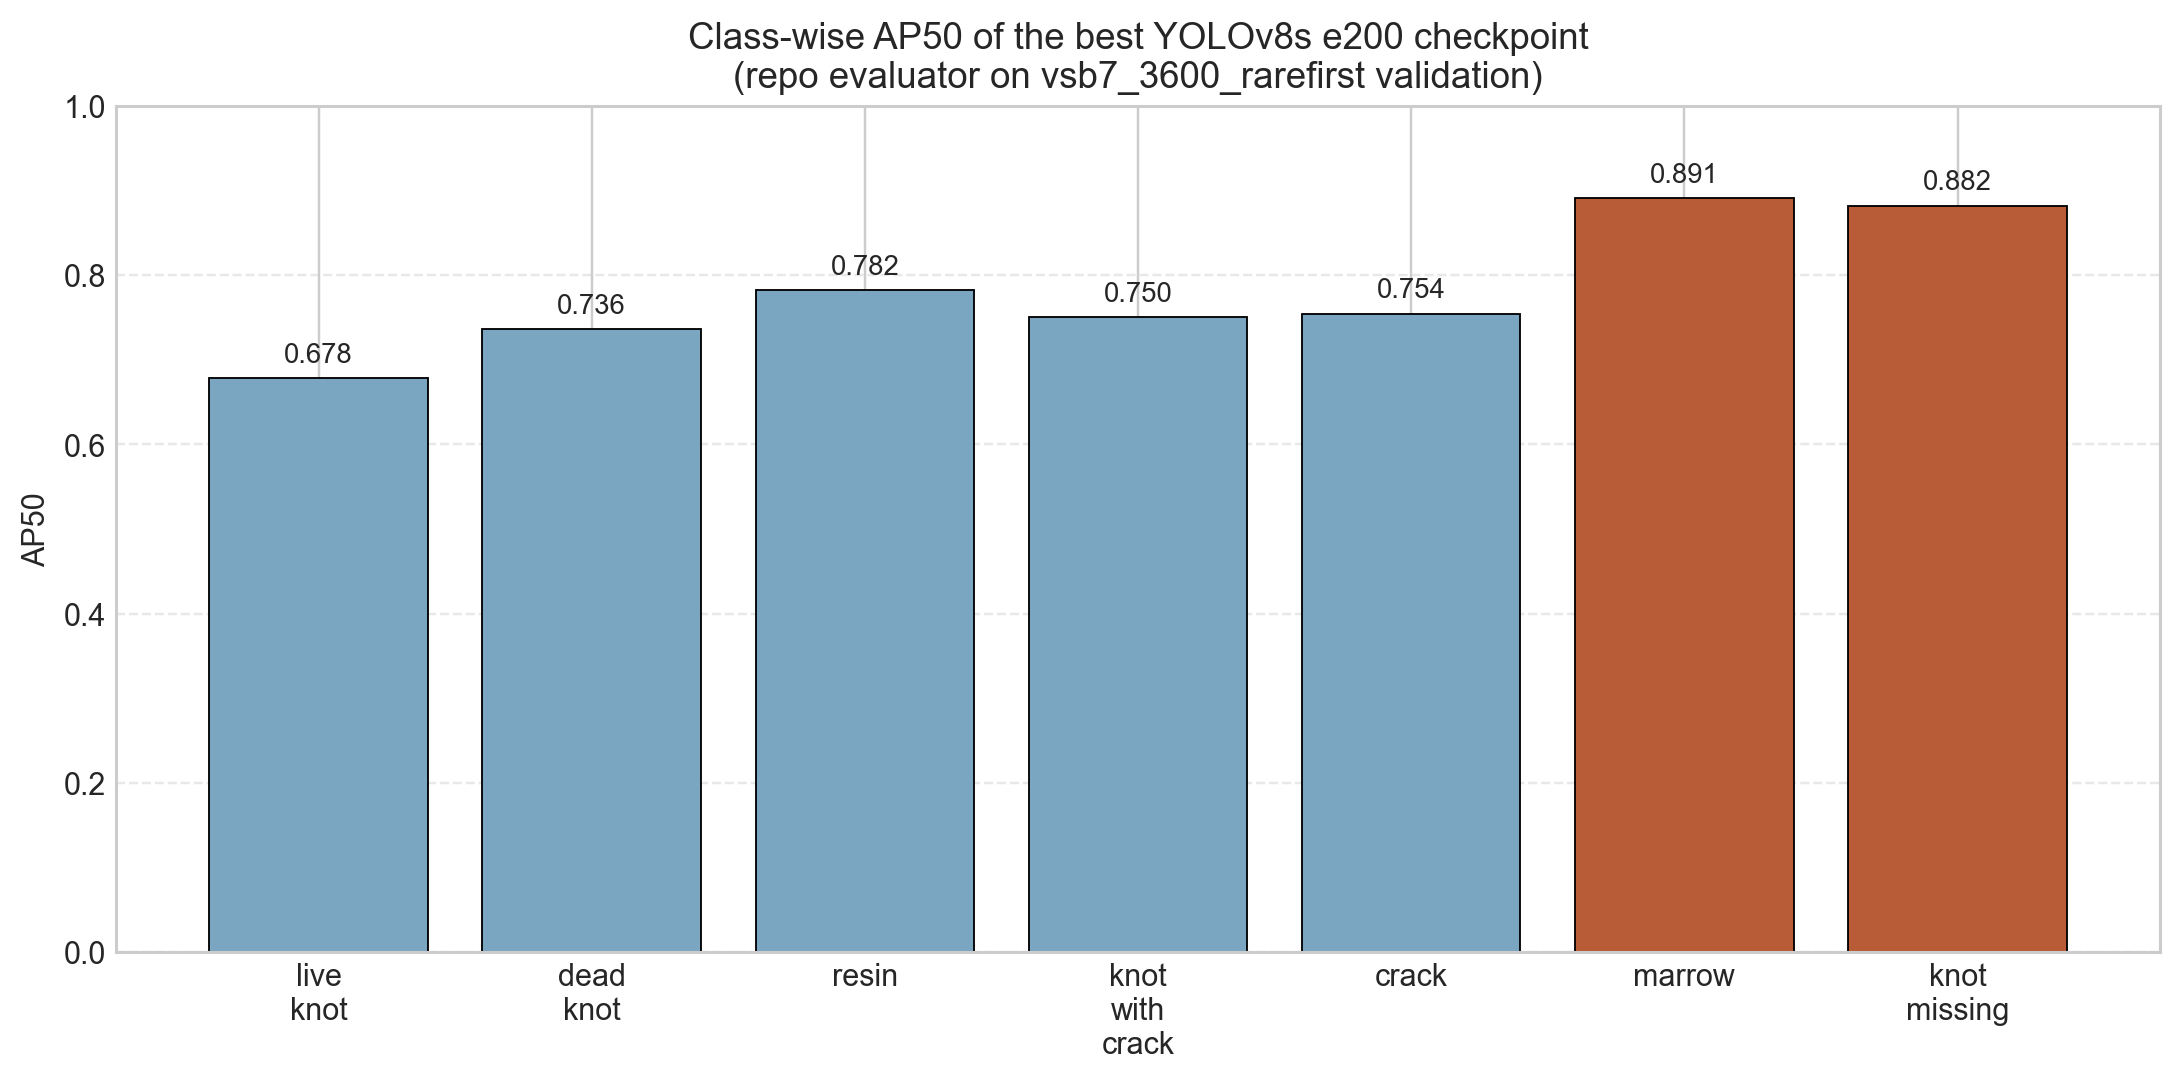
\includegraphics[width=0.90\linewidth]{figures/y0_3600_classwise_ap50.png}
  \caption{Class-wise AP50 of the saved best \texttt{Y0-3600e200} checkpoint under the unified study evaluator on the screened validation split. This figure is used as a diagnostic label-wise view of the final 200-epoch model.}
  \label{fig:y0-classwise-ap50}
\end{figure}

Figure~\ref{fig:yolo-progress} shows the training dynamics of the 200-epoch screened YOLOv8s run. The curve rises rapidly during the early schedule, reaches its highest AP50 at epoch 55, and then remains stable without major degradation. This behavior provides a stronger long-schedule confirmation of the selected compact baseline and a more credible comparison point against recent public YOLO-based studies than the short screening runs alone.

\begin{figure*}[t]
  \centering
  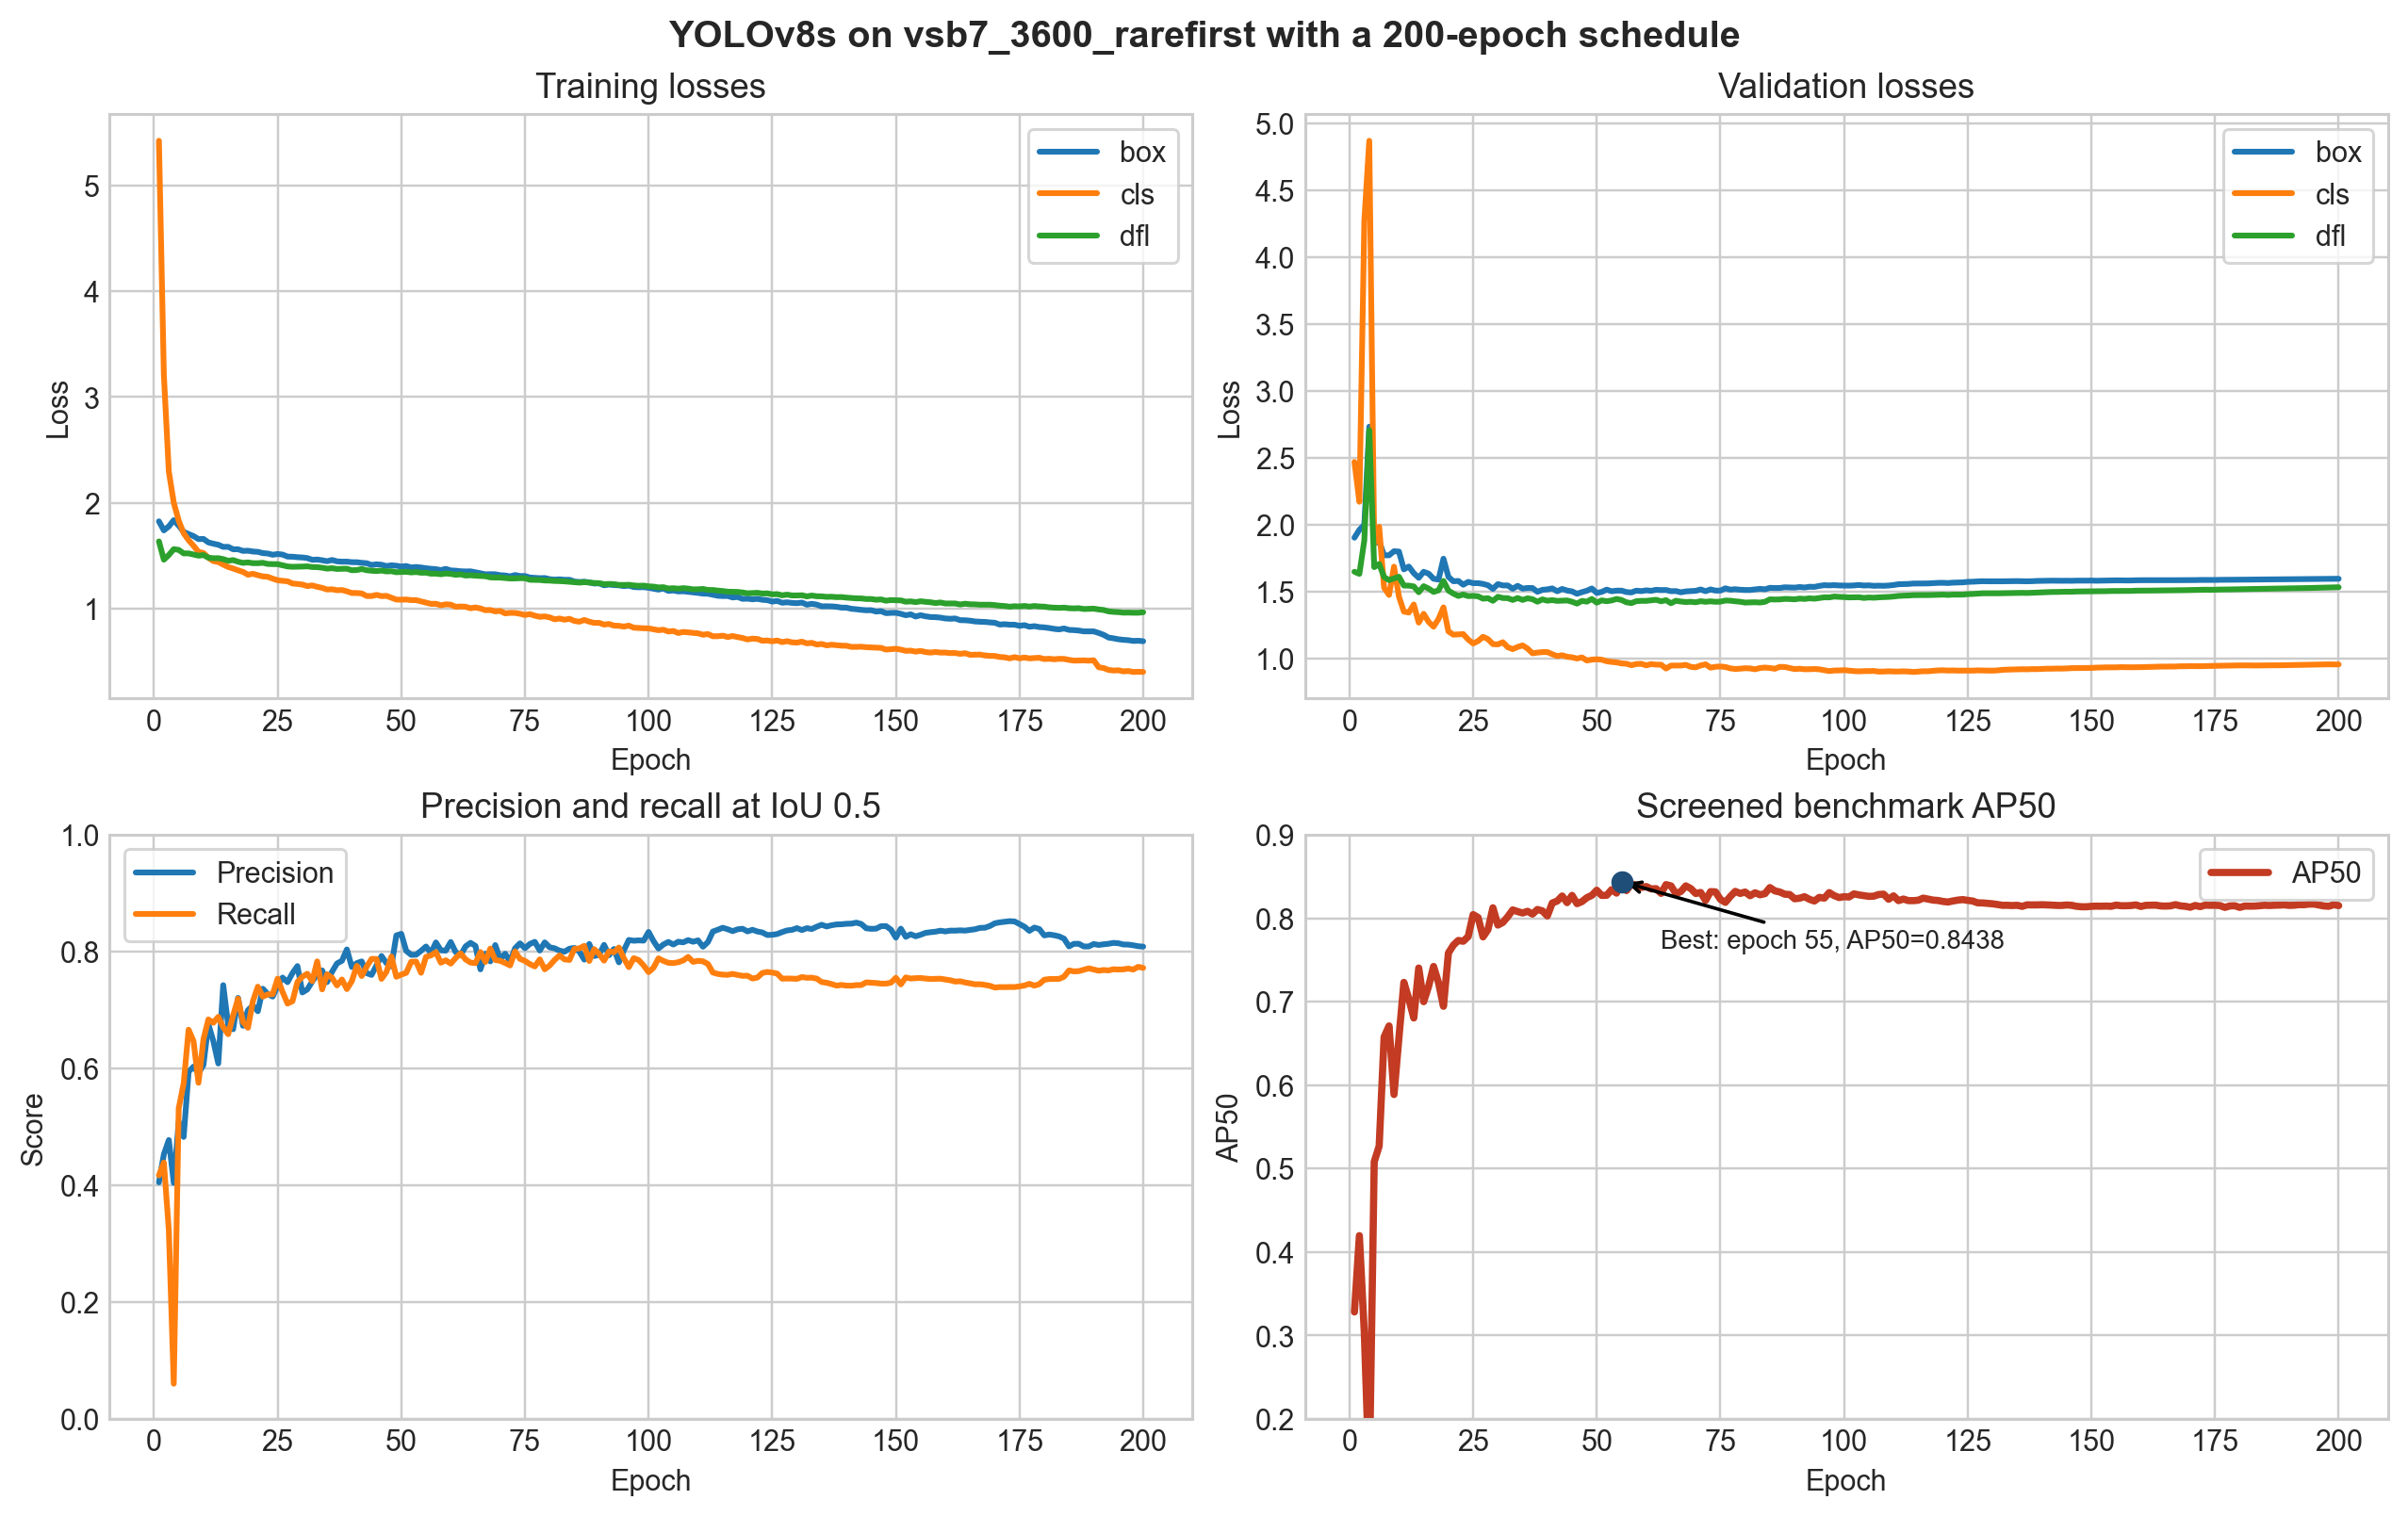
\includegraphics[width=0.92\linewidth]{figures/yolo_protocol_progress.png}
  \caption{Training progress of the 200-epoch screened YOLOv8s run. The model reaches its best AP50 at epoch 55 and then stays in a stable high-performance regime, which supports using this run for literature-facing comparison.}
  \label{fig:yolo-progress}
\end{figure*}

\subsection{Target-Domain Adaptation Results on VNWoodKnot}
\label{sec:external-results}

Table~\ref{tab:external} summarizes short-budget target-domain adaptation on VNWoodKnot.
Three results are notable:

\begin{itemize}[leftmargin=1.5em]
  \item On the held-out target-domain test split, \texttt{T1} reaches 0.8312 AP50, whereas \texttt{T0} reaches 0.7753. This is a gain of 5.59 AP50 points under the same 50-epoch adaptation budget.
  \item \texttt{T1} is also cleaner: precision improves from 0.5370 to 0.6730 while recall improves from 0.8903 to 0.9161, and the total number of predictions drops from 257 to 211.
  \item The validation trajectories still show an optimization advantage for source initialization. \texttt{T1} reaches 0.70 AP50 by epoch 9 and 0.80 by epoch 31, whereas \texttt{T0} reaches the same thresholds only at epochs 19 and 40, respectively.
\end{itemize}

These results indicate that the target task is learnable within a modest training budget and that the screened-source checkpoint acts as a useful initializer rather than merely as a faster warm start. In other words, the external question becomes less about whether the target task can be learned at all and more about how much target-domain supervision is needed to convert source-domain knowledge into held-out target-domain gains.

\begin{table}[t]
  \centering
  \caption{Target-domain adaptation on VNWoodKnot under a fixed 50-epoch budget. Results are reported on the held-out target-domain test split using the best checkpoint selected within each 50-epoch run.}
  \label{tab:external}
  \footnotesize
  \setlength{\tabcolsep}{4pt}
  \begin{tabularx}{\linewidth}{>{\raggedright\arraybackslash}p{0.10\linewidth} >{\raggedright\arraybackslash}p{0.23\linewidth} c c c X}
    \toprule
    ID & Setting & AP50 & Prec.50 & Rec.50 & Notes \\
    \midrule
    \texttt{T0} & target-only supervised training & 0.7753 & 0.5370 & 0.8903 & held-out test, 257 predictions \\
    \texttt{T1} & \texttt{Y0-3600e200} $\rightarrow$ fine-tune & \best{0.8312} & \best{0.6730} & \best{0.9161} & held-out test, 211 predictions \\
    \bottomrule
  \end{tabularx}
\end{table}

Figure~\ref{fig:vnwoodknot-transfer} visualizes the same pattern. The left panel shows held-out test AP50 overall and by class. The largest gain comes from \texttt{live\_knot}, where AP50 rises from 0.7106 to 0.8324. For \texttt{dead\_knot}, AP50 stays nearly unchanged, but precision and recall still improve. The right panel shows the first 50 validation epochs and confirms that \texttt{T1} enters a useful accuracy regime much earlier than \texttt{T0}. Together, these two views show that the screened source checkpoint improves both optimization speed and final held-out target-domain performance.

\begin{figure}[t]
  \centering
  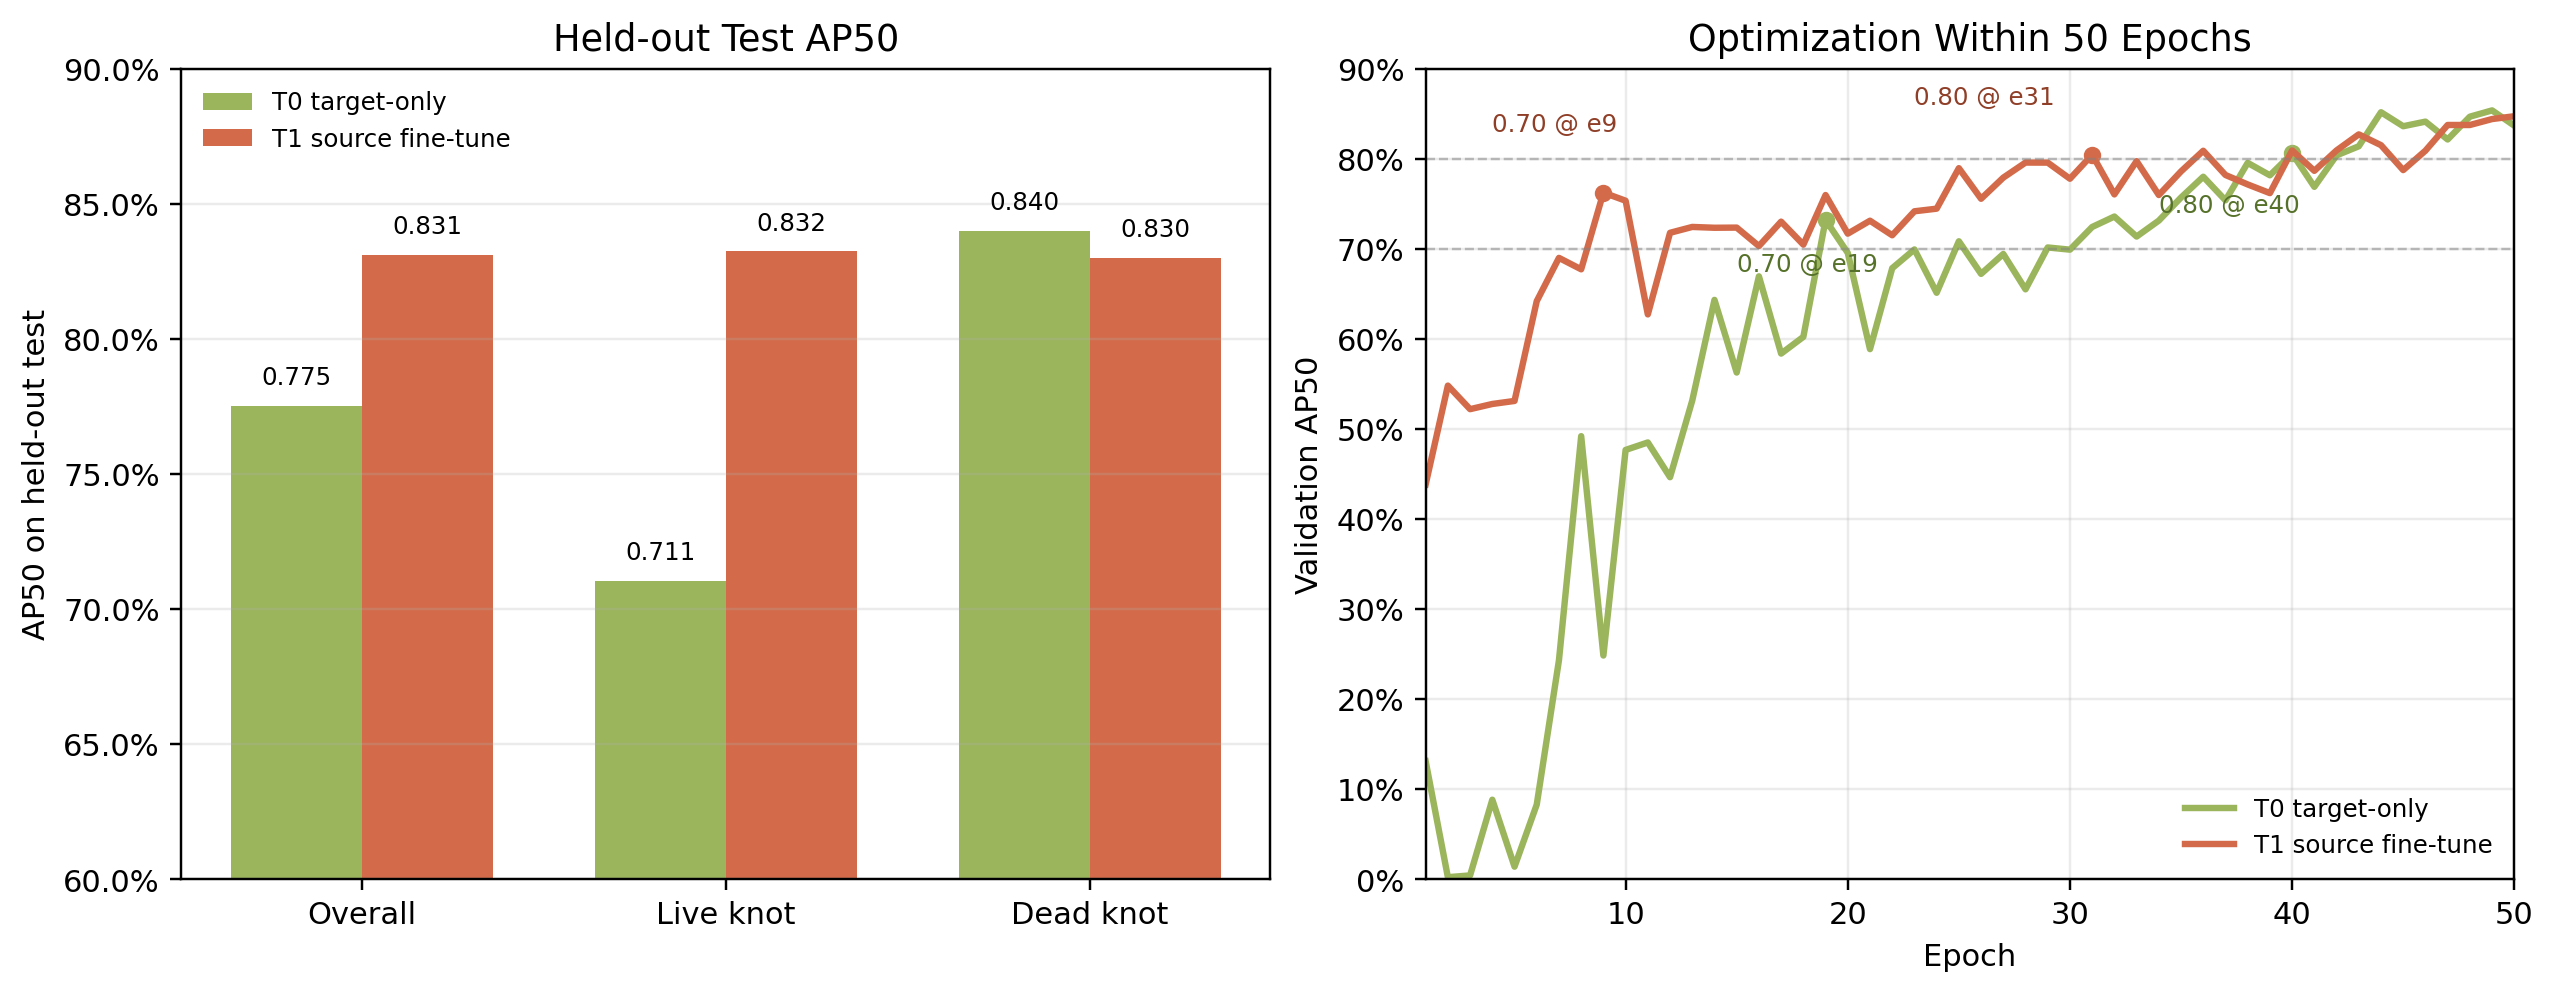
\includegraphics[width=0.98\linewidth]{figures/vnwoodknot_adaptation_50e.png}
  \caption{VNWoodKnot adaptation under a fixed 50-epoch budget. Left: held-out test AP50 overall and by class for target-only training and screened-source fine-tuning. Right: validation AP50 trajectories for the first 50 epochs.}
  \label{fig:vnwoodknot-transfer}
\end{figure}

\section{Discussion}
\label{sec:discussion}

The results presented in Section~\ref{sec:experiments} support three main observations. First, a compact YOLOv8s baseline remains stronger than all other tested detector choices in the present design space, and the 200-epoch screened run makes this conclusion much sharper. The distinction between the short screening stage and the long-schedule confirmation run is important here. The 20-epoch runs are used to compare detector families and local refinements inside the study, whereas the 200-epoch screened YOLOv8s run is used as the final literature-facing benchmark result. Once the strongest compact baseline is trained with a longer schedule, its AP50 reaches 84.38\% and moves above the values reported by the most comparable recent public screened-benchmark studies. In practical terms, this means that a carefully optimized compact baseline can remain highly competitive, and in our case even stronger than several recent custom detector variants, without requiring a heavier model or an additional architectural block. We still do not treat this as an unconditional SOTA claim because the reconstructed benchmark, checkpoint policy, and evaluation details are not perfectly identical across studies. Even so, the result is strong enough to support a clear claim of public-level competitiveness, and likely superiority, on the screened benchmark used in this study.

Second, detector-family selection matters more than local detector refinement. The Faster R-CNN + MobileNet family remains useful as a lightweight reference and provides an important engineering baseline. However, the tested MobileNet-based runs do not match the compact YOLOv8s baseline on either the screened benchmark or the broader full seven-class protocol. Likewise, the P2-head and WNIoU-style refinements do not improve the compact baseline in the study-internal 20-epoch screening stage. This combination of results changes the optimization target. If the detector family itself is already stronger, then simple head-level modification or loss substitution may add complexity without changing the overall ranking. In our study, the practical progression is therefore from lightweight two-stage exploration toward a compact one-stage baseline.

Third, benchmark breadth and domain shift remain the real constraints on deployment. Even with the stronger 200-epoch screened result, the broader full seven-class protocol remains lower. In native YOLO validation, the additional full-protocol rerun improves only marginally from 80.39\% to 81.16\% AP50, while under the unified study evaluator it does not improve the stronger 20-epoch internal reference. This means that the screened-benchmark advantage is not explained away by schedule length alone. The VNWoodKnot adaptation results make the same point from a different angle: a source-domain prior helps, but only once target-domain supervision is introduced. Taken together, these findings suggest that our main challenge is no longer finding a detector that scores well on one curated split. The harder challenge is to preserve or recover that performance once the protocol broadens or the data source changes.

The ablation results also help clarify what is \emph{not} currently limiting performance. The P2-head modification is motivated by common small-object detection heuristics, and the WNIoU-style loss is motivated by the difficulty of localizing small or visually weak defects. Nevertheless, neither modification improves AP50 over the YOLOv8s baseline in our experiments. These negative results are still informative. They suggest that, under the current dataset, label space, and training recipe, the main bottleneck is not simply the absence of a higher-resolution detection head or a single alternative regression-loss term. This does not imply that such changes are universally ineffective; rather, it indicates that they are insufficient by themselves within the present protocol.

The VNWoodKnot results provide a useful practical counterpart to the in-domain findings. When these results are interpreted together with the dataset analysis and the first 50 epochs of supervised target-domain training, the most defensible conclusion is that domain shift remains substantial, but the screened source checkpoint still offers a useful adaptation prior. VNWoodKnot differs from the in-domain dataset in label space, object scale, image framing, and small-defect prevalence. These differences make cross-domain reuse nontrivial. At the same time, once supervised target-domain training is allowed, the source-initialized model now shows a held-out performance gain rather than merely a faster warm start. On the target-domain test split, \texttt{T1} reaches 83.12\% AP50, while \texttt{T0} reaches 77.53\%, with both precision and recall improving. The largest AP50 gain appears on \texttt{live\_knot}, where transfer sharply reduces false positives without sacrificing recall. This does not imply that the transfer problem is fully solved; rather, it suggests that the screened source checkpoint is helpful as a practical starting point for supervised adaptation under a limited budget. The additional observation that the earlier MobileNet-based detector also collapses externally reinforces the broader interpretation that detector-family choice alone is not enough to neutralize cross-domain mismatch.

This study still has several limitations. The current in-domain matrix remains single-seed, so a final journal version should report mean $\pm$ std over three seeds for the main baselines (\texttt{Y0-full} and \texttt{Y0-3600e200}), and ideally for the ablations (\texttt{Y1} and \texttt{Y2}) as well. In addition, the broader full seven-class protocol and the auxiliary screened controls have not yet been rerun under the same 200-epoch budget as the final screened benchmark result, with the exception of the diagnostic \texttt{Y0-full\_e200} check reported here. For that reason, the 84.38\% AP50 run is best interpreted as the current final literature-facing screened result, while the 20-epoch rows for \texttt{Y0-full}, \texttt{Y1}, and \texttt{Y2} should still be read as study-internal screening comparisons pending longer-schedule updates. The present paper also combines native YOLO validation for literature-facing comparisons with the unified study evaluator for cross-family and external analyses; this distinction is now explicit, but a cleaner final version would benefit from fully harmonized metric reporting wherever possible. The present paper also does not yet report matched latency and memory benchmarks across the Faster R-CNN and YOLO branches, meaning that the ``resource-aware'' framing should be read as a detector-selection study rather than as a finalized embedded-deployment benchmark. For the external setting, the supervised adaptation comparison is intentionally limited to a 50-epoch budget, so the present evidence should be read as a short-budget adaptation result rather than as a full convergence study. A complete journal version should still add the pending full-source transfer run from \texttt{Y0-full} (\texttt{T2}) and multi-seed repeats for the VNWoodKnot adaptation setting. These directions are important for strengthening the practical implications of the present findings.
